\documentclass[12pt]{article}
\usepackage{float}
\usepackage[ruled,vlined,linesnumbered,algo2e]{algorithm2e}
\usepackage{amsmath,amssymb}
\usepackage{amsthm}
\usepackage{makecell}
\usepackage{subcaption}

\usepackage{pgfplots}
% and optionally (as of Pgfplots 1.3):
\pgfplotsset{compat=newest}
\pgfplotsset{plot coordinates/math parser=false}
\newlength\figureheight
\newlength\figurewidth


\usepackage[a4paper, total={6.5in, 9in}]{geometry}
\usepackage{tikz}
\newcommand*\circled[1]{\tikz[baseline=(char.base)]{
   \node[shape=circle,draw=red,inner sep=1pt] (char) {#1};}}
\setlength\parindent{0pt} %% Do not touch this
\DeclareMathOperator{\phiAb}{\phi_{A,\mathbf{b}}}
\DeclareMathOperator*{\argmax}{arg\,max}
\DeclareMathOperator*{\argmin}{arg\,min}
\newtheorem{lemma}{Lemma}
\newtheorem{theorem}{Theorem}
\newtheorem{definition}{Definition}
%% -----------------------------
%% TITLE
%% -----------------------------
\title{Short review of different beamforming techniques for passive array processing} %% Assignment Title
\author{Wissal Ghamour, Julien Gleyze and Nathan Rousselot}
%% Change "\today" by another date manually
%% -----------------------------
%% -----------------------------

%% %%%%%%%%%%%%%%%%%%%%%%%%%
\begin{document}
%\setlength{\droptitle}{-5em}    
%% %%%%%%%%%%%%%%%%%%%%%%%%%
\maketitle
% --------------------------
% Start here
% --------------------------
\section{Introduction}
In this document, we will cover a range of techniques specific to array processing. Array processing is a branch of signal processing dedicated to the processing of signals produced or received by an array of elements. Those element can be antennas in passive setups, or transducers in the context of radar or sonar processing. In the following, we will focus on the passive setup, meaning we work with an array of sensors. This class of problem has a wide range of applications, from radio astronomy to wireless communications. All those applications share common challenges, such as the estimation of the direction of arrival (DOA) of a signal, or optimizing the Signal-to-Interference-plus-Noise ratio (SINR). In this introductory document, we will focus ourselves on the impact of the choice of beamforming techniques, ranging from Conventional Beamforming to more robust and adaptative methods.
\section{Direct Methods}
Consider the following signal
\begin{equation}\label{eq:signal}
   \mathbf{y}(k) = \mathbf{a}_ss(k) + \mathbf{y}_{I}(k) + \mathbf{n}(k)
\end{equation}
where $\mathbf{a}_s$ is the steering vector of the signal of interest, $s(k)$ is the signal of interest, $\mathbf{y}_{I}(k)$ is the interference signal, and $\mathbf{n}(k)$ is the noise. In this section, it is assumed that $\mathbf{a}_s$ is perfectly known, meaning $\mathbf{a}_0 = \mathbf{a}_s$. The goal of beamforming is to find a weight vector $\mathbf{w}$ such that the output of the beamformer $\hat{s}(k)$ is a good estimate of $s(k)$. The output of the beamformer is given by
\begin{equation}\label{eq:bf}
   \hat{s}(k) = \mathbf{w}^H\mathbf{y}(k)
\end{equation}
\subsection{Conventional Beamformer}
The conventional beamformer is the simplest beamformer. It is defined as
\begin{equation}\label{eq:cbf}
   \mathbf{w}_{CBF} \propto \mathbf{a}(\theta_s)
\end{equation}
\begin{theorem}
    Let $\mathbf{y}(k)$ be defined by equation \ref{eq:signal} and $\mathbf{w}$ the weight vector. Considering $\mathbf{a}^H(\theta_s)\mathbf{a}(\theta_s)$ is non-singular, the coefficients of $\mathbf{w}$ that maximize the gain at $\theta_s$, subject to equation \ref{eq:cbf} is given by
    \begin{equation}
        \mathbf{w}_{CBF} = \left(\mathbf{a}^H(\theta_s)\mathbf{a}(\theta_s)\right)^{-1}\mathbf{a}(\theta_s)
    \end{equation}
\end{theorem}
\begin{proof}

\end{proof}
This beamformer is optimal when there is no-noise, and no-interference. In the vast majority of applications, this is obviously not the case. 
\subsection{Optimal Adaptative Beamformer}\label{sec:opt}
In actual conditions, CBF will prove itself as very sub-optimal. In this section we will introduce a new beamformer, that is deemed and called ``optimal''. It accounts for interferences and noise, thus fitting the model depicted in equation \ref{eq:signal}. Let us formulate this as an optimization problem. Let $\mathbf{w}\in\mathcal{W}$, the weight vector, then
\begin{equation}
    \mathbf{w}_{opt} = \max_{w\in\mathcal{W}}  \text{ SINR}(\mathbf{w})
\end{equation}
\begin{theorem}\label{thm:wopt}
    Let $\mathbf{y}(k)$ be defined following equation \ref{eq:signal} of length N. Assuming that $\forall k, \lambda_k(\mathbf{y}_I(k)+\mathbf{n}(k)) \neq 0$, with $\lambda_k(\mathbf{A})$ eigenvalues of $\mathbf{A}$, then 
    \begin{equation}\label{eq:wopt}
        \mathbf{w}_{opt} = \frac{\mathbf{C}^{-1}\mathbf{a}_s}{\mathbf{a}_s^H\mathbf{C}^{-1}\mathbf{a}_s}
    \end{equation}
\end{theorem}
\begin{proof}
From equations \ref{eq:signal} and \ref{eq:bf}, one can rewrite the output of the beamformer as
\begin{equation*}\label{eq:new_signal}
   \hat{s}(k) = \mathbf{w}^H\mathbf{a}_ss(k) + \mathbf{w}^H\mathbf{y}_{I}(k) + \mathbf{w}^H\mathbf{n}_k
\end{equation*}
\begin{equation*}
    \Rightarrow \text{ SINR}(\mathbf{w}) = \frac{\mathbb{E}\left[|\mathbf{w}^H\mathbf{a}_ss(k)|^2\right]}{\mathbb{E}\left[|\mathbf{w}^H\mathbf{y}_{I}(k) + \mathbf{w}^H\mathbf{n}(k)|^2\right]} = \frac{P_s|\mathbf{w}^H\mathbf{a}_s|^2}{\mathbf{w}^H\mathbf{C}\mathbf{w}}
\end{equation*}
Where $\mathbf{C}$ is the noise plus interference covariance matrix.
It is assumed that $\forall k, \lambda_k(\mathbf{C})\neq 0$. Thus, equation \ref{eq:wopt} rewrites
\begin{equation*}
    \mathbf{w}_{opt} = \max_{w\in\mathcal{W}} \frac{P_s|\mathbf{w}^H\mathbf{a}_s|^2}{\mathbf{w}^H\mathbf{C}\mathbf{w}}
\end{equation*}
For practical reason, let us constrain the gain to be unit
$$\begin{aligned}
    \mathbf{w}_{opt} =& \max_{w\in\mathcal{W}} &\frac{P_s|\mathbf{w}^H\mathbf{a}_s|^2}{\mathbf{w}^H\mathbf{C}\mathbf{w}}\\
    & \textrm{s.t.} \quad &|\mathbf{w}^H\mathbf{a}_s| = 1
\end{aligned} \Longleftrightarrow \begin{aligned}
    \mathbf{w}_{opt} =& \max_{w\in\mathcal{W}} &\frac{P_s}{\mathbf{w}^H\mathbf{C}\mathbf{w}}\\
    & \textrm{s.t.} \quad &|\mathbf{w}^H\mathbf{a}_s| = 1
\end{aligned}$$
Which yiels the following optimization problem
$$\begin{aligned}
    \mathbf{w}_{opt} =& \min_{w\in\mathcal{W}} &\mathbf{w}^H\mathbf{C}\mathbf{w}\\
    & \textrm{s.t.} \quad &|\mathbf{w}^H\mathbf{a}_s| = 1
\end{aligned}$$
\end{proof}
% %%%%%%%%%%%%%%%%%%%
\section{Practical Adaptative Beamforming Techniques}
In reality, the optimal beamformer (section \ref{sec:opt}) is very unpractical. Indeed, in actual conditions, the steering vector $\mathbf{a}_s$ and the covariance matrix $\mathbf{C}$ are unknown. Instead, we have approximates, respectively $\mathbf{a}_0$ and $\hat{\mathbf{C}}$.
\subsection{Minimum Variance Distortionless Response}
The Minimum Variance Distortionless Responsor (MVDR) is the direct consequence of the optimal beamformer (section \ref{sec:opt}) with approximated entries. It thus writes automatically
\begin{equation}\label{eq:mvdr}
    \mathbf{w}_{mvdr}^{smi} = \frac{\hat{\mathbf{C}}^{-1}\mathbf{a}_0}{\mathbf{a}_0^H\hat{\mathbf{C}}^{-1}\mathbf{a}_0}
\end{equation}
where $smi$ stands for ``sample matrix inversion'' and is directly linked to how $\hat{\mathbf{C}}$ is being approximated (equation \ref{eq:chat}).
\begin{equation}\label{eq:chat}
    \hat{\mathbf{C}} = \frac{1}{K}\sum_{k=1}^K \mathbf{y}(k)\mathbf{y}^H(k)
\end{equation}
where $\mathbf{y}(k) = \mathbf{y}_I(k)+\mathbf{n}(k)$
\subsection{Minimum Power Distortionless Response}
\subsubsection{Naive Approach}
Sometimes, it is not possible to isolate the noise and the interference to estimate $\mathbf{C}$. Leading us to the Minimum Power Distortionless Response beamformer (MPDR).
\begin{equation}\label{eq:mvdr}
    \mathbf{w}_{mpdr}^{smi} = \frac{\hat{\mathbf{R}}^{-1}\mathbf{a}_0}{\mathbf{a}_0^H\hat{\mathbf{R}}^{-1}\mathbf{a}_0}
\end{equation}

\begin{equation}\label{eq:chat}
    \hat{\mathbf{R}} = \frac{1}{K}\sum_{k=1}^K \mathbf{y}(k)\mathbf{y}^H(k)
\end{equation}
where $\mathbf{y}(k) = \mathbf{a}_ss(k) + \mathbf{y}_I(k)+\mathbf{n}(k)$. Intuitively, one can think that adding the signal information to the covariance matrix will lead to signal degradation as we want to minimize its output power. 
\begin{lemma}\label{lem:mpdr}
    In case where $K\rightarrow\infty$ and $\mathbf{a}_0 = \mathbf{a}_s$, then the beam patterns of MVDR and MPDR are identical.
\end{lemma}
\begin{proof}
    Recall from equation \ref{eq:bf}
    \begin{equation*}
        \hat{s}(k)=\mathbf{w}^H\mathbf{a}_ss(k) + \mathbf{w}^H\mathbf{y}_I(k) + \mathbf{w}^H\mathbf{n}(k)
    \end{equation*}
    Now recall from Theorem \ref{thm:wopt} 
    $$\begin{aligned}
    \mathbf{w} =& \min_{w\in\mathcal{W}} &\mathbf{w}^H\mathbf{C}\mathbf{w}\\
    & \textrm{s.t.} \quad &|\mathbf{w}^H\mathbf{a}_s| = 1
\end{aligned}$$
    The constraint $|\mathbf{w}^H\mathbf{a}_s| = 1$ then ensures that the part of $\hat{s(k)}$ with the signal of interest will be preserved.
\end{proof}
In lemma \ref{lem:mpdr}, we demonstrated that MPDR and MVDR are equivalent mathematically, even while having different formulations. However, it is based uppon two strong assumptions, that are, in practice, very unrealistic. We will analyze the impact of releasing the constraint on $K$ and on $\mathbf{a_0}$ seperately.

Figure \ref{fig:mpdr_robust} illustrate the lack of robustness in MPDR method, with respect to error in the direction of arrival estimation $\Delta\theta$. It shows from figure \ref{fig:mpdr_robus_sinr} that the resulting SINR with MPDR is greatly suboptimal as soon as $\Delta\theta$ increases a bit. Looking at the array white noise gain $A_{WN}$ (figure \ref{fig:mpdr_robus_awn}, we observe that this gain dramatically decreases as $\Delta\theta$ increases. Recall that 
\begin{equation}
    A_{WN} = \|w\|^{-2} \leq N
\end{equation}
Ideally, we would want $A_{WN}=N$, and thus the pattern drawn in figure \ref{fig:mpdr_robus_awn} is worrying.
\begin{figure}[H]
    \centering
    \begin{subfigure}[b]{.4\linewidth}
        % This file was created by matlab2tikz.
%
%The latest updates can be retrieved from
%  http://www.mathworks.com/matlabcentral/fileexchange/22022-matlab2tikz-matlab2tikz
%where you can also make suggestions and rate matlab2tikz.
%
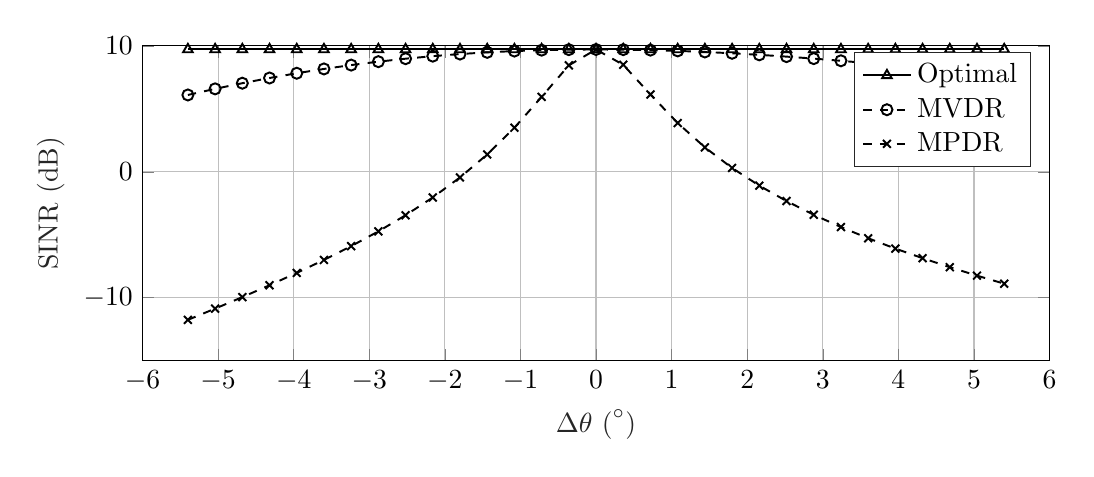
\begin{tikzpicture}

\begin{axis}[%
width=.95\linewidth,
height=4cm,
at={(0in,0in)},
scale only axis,
xmin=-6,
xmax=6,
xlabel style={font=\color{white!15!black}},
xlabel={$\Delta\theta\text{ (}^\circ\text{)}$},
ymin=-15,
ymax=10,
ylabel style={font=\color{white!15!black}},
ylabel={SINR (dB)},
axis background/.style={fill=white},
title style={font=\bfseries},
%title={MVDR vs MPDR vs Optimal : SINR Comparison in function of DOA error},
xmajorgrids,
ymajorgrids,
legend style={legend cell align=left, align=left, draw=white!15!black}
]
\addplot [color=black, line width=0.7pt, mark=triangle, mark options={solid, black}]
  table[row sep=crcr]{%
-5.4	9.71005093279693\\
-5.04	9.71005093279693\\
-4.68	9.71005093279693\\
-4.32	9.71005093279693\\
-3.96	9.71005093279693\\
-3.6	9.71005093279693\\
-3.24	9.71005093279693\\
-2.88	9.71005093279693\\
-2.52	9.71005093279693\\
-2.16	9.71005093279693\\
-1.8	9.71005093279693\\
-1.44	9.71005093279693\\
-1.08	9.71005093279693\\
-0.72	9.71005093279693\\
-0.36	9.71005093279693\\
0	9.71005093279693\\
0.36	9.71005093279693\\
0.72	9.71005093279693\\
1.08	9.71005093279693\\
1.44	9.71005093279693\\
1.8	9.71005093279693\\
2.16	9.71005093279693\\
2.52	9.71005093279693\\
2.88	9.71005093279693\\
3.24	9.71005093279693\\
3.6	9.71005093279693\\
3.96	9.71005093279693\\
4.32	9.71005093279693\\
4.68	9.71005093279693\\
5.04	9.71005093279693\\
5.4	9.71005093279693\\
};
\addlegendentry{Optimal}

\addplot [color=black, dashed, line width=0.7pt, mark=o, mark options={solid, black}]
  table[row sep=crcr]{%
-5.4	6.09852443082549\\
-5.04	6.58337563304574\\
-4.68	7.03218680480885\\
-4.32	7.44518430075109\\
-3.96	7.82249333838131\\
-3.6	8.1642038737273\\
-3.24	8.47043019281701\\
-2.88	8.74136297639043\\
-2.52	8.97731227175406\\
-2.16	9.17873985492887\\
-1.8	9.34627986364081\\
-1.44	9.48074725330597\\
-1.08	9.58313445536689\\
-0.72	9.65459745669455\\
-0.36	9.69643323107577\\
0	9.71005093279693\\
0.36	9.69693945416944\\
0.72	9.65863385691013\\
1.08	9.59668286275238\\
1.44	9.51261911163404\\
1.8	9.40793335390064\\
2.16	9.2840532135159\\
2.52	9.14232669842924\\
2.88	8.98401027358856\\
3.24	8.81026106096857\\
3.6	8.62213258228707\\
3.96	8.4205733967394\\
4.32	8.20642798693983\\
4.68	7.9804392903552\\
5.04	7.74325234263035\\
5.4	7.49541857901868\\
};
\addlegendentry{MVDR}

\addplot [color=black, dashed, line width=0.7pt, mark=x, mark options={solid, black}]
  table[row sep=crcr]{%
-5.4	-11.7526261836208\\
-5.04	-10.8602186360387\\
-4.68	-9.94706192248612\\
-4.32	-9.00514749410739\\
-3.96	-8.02510108488326\\
-3.6	-6.99563324182524\\
-3.24	-5.90277054213023\\
-2.88	-4.72875214169016\\
-2.52	-3.45042127447117\\
-2.16	-2.03689277275537\\
-1.8	-0.44638168633892\\
-1.44	1.37690336621313\\
-1.08	3.49906300741658\\
-0.72	5.94850519209378\\
-0.36	8.44974234211841\\
0	9.71005093279688\\
0.36	8.49066107419558\\
0.72	6.13678043996599\\
1.08	3.87192119044684\\
1.44	1.93851857012253\\
1.8	0.303132095086112\\
2.16	-1.09949811334601\\
2.52	-2.32353255496334\\
2.88	-3.40919948950323\\
3.24	-4.38597512035512\\
3.6	-5.27570073314045\\
3.96	-6.09485411479017\\
4.32	-6.85610721125907\\
4.68	-7.5693869967579\\
5.04	-8.24260557578834\\
5.4	-8.8821709464785\\
};
\addlegendentry{MPDR}

\end{axis}
\end{tikzpicture}%
        \caption{SINR vs error in $\mathbf{a}_0$}
        \label{fig:mpdr_robus_sinr}
    \end{subfigure}\hspace{0.09\linewidth}
    \begin{subfigure}[b]{.4\linewidth}
        % This file was created by matlab2tikz.
%
%The latest updates can be retrieved from
%  http://www.mathworks.com/matlabcentral/fileexchange/22022-matlab2tikz-matlab2tikz
%where you can also make suggestions and rate matlab2tikz.
%
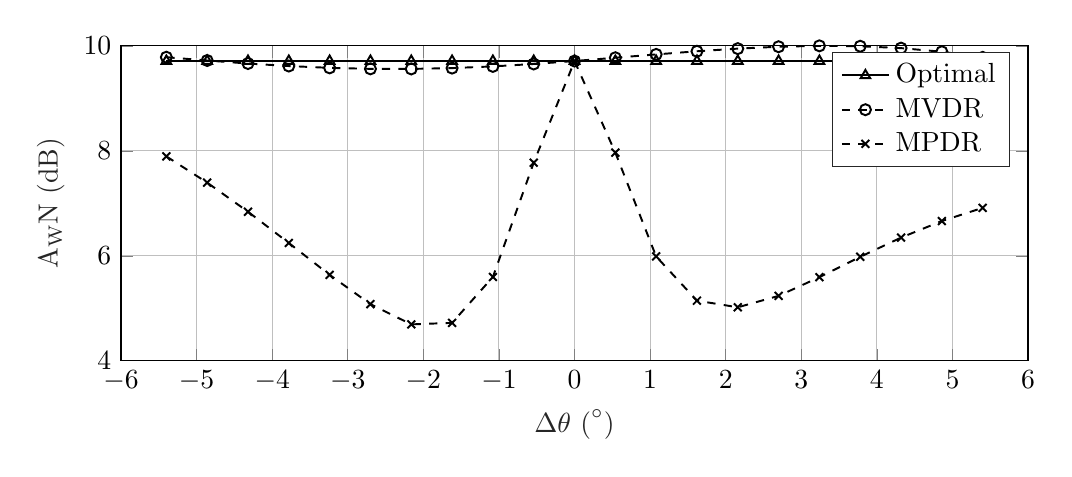
\begin{tikzpicture}

\begin{axis}[%
width=.95\linewidth,
height=4cm,
at={(0in,0in)},
scale only axis,
xmin=-6,
xmax=6,
xlabel style={font=\color{white!15!black}},
xlabel={$\Delta\theta\text{ (}^\circ\text{)}$},
ymin=4,
ymax=10,
ylabel style={font=\color{white!15!black}},
ylabel={$\text{A}_\text{W}\text{N (dB)}$},
axis background/.style={fill=white},
title style={font=\bfseries},
%title={$\text{MVDR vs MPDR vs Optimal : A}_\text{W}\text{N Comparison in function of DOA error}$},
xmajorgrids,
ymajorgrids,
legend style={legend cell align=left, align=left, draw=white!15!black}
]
\addplot [color=black, line width=0.7pt, mark=triangle, mark options={solid, black}]
  table[row sep=crcr]{%
-5.4	9.71035096166965\\
-4.86	9.71035096166965\\
-4.32	9.71035096166965\\
-3.78	9.71035096166965\\
-3.24	9.71035096166965\\
-2.7	9.71035096166965\\
-2.16	9.71035096166965\\
-1.62	9.71035096166965\\
-1.08	9.71035096166965\\
-0.54	9.71035096166965\\
0	9.71035096166965\\
0.54	9.71035096166965\\
1.08	9.71035096166965\\
1.62	9.71035096166965\\
2.16	9.71035096166965\\
2.7	9.71035096166965\\
3.24	9.71035096166965\\
3.78	9.71035096166965\\
4.32	9.71035096166965\\
4.86	9.71035096166965\\
5.4	9.71035096166965\\
};
\addlegendentry{Optimal}

\addplot [color=black, dashed, line width=0.7pt, mark=o, mark options={solid, black}]
  table[row sep=crcr]{%
-5.4	9.78281284253418\\
-4.86	9.72013279596549\\
-4.32	9.66262710141472\\
-3.78	9.61468387867466\\
-3.24	9.57995946107594\\
-2.7	9.56111867353351\\
-2.16	9.55962385200562\\
-1.62	9.57561000567684\\
-1.08	9.6078698875444\\
-0.54	9.65395178226749\\
0	9.71035096166965\\
0.54	9.77275983937592\\
1.08	9.83633599890023\\
1.62	9.89595140919136\\
2.16	9.94639686132814\\
2.7	9.98252837530016\\
3.24	9.99935330789475\\
3.78	9.99206121255362\\
4.32	9.95600790104479\\
4.86	9.88666137187009\\
5.4	9.77951633382353\\
};
\addlegendentry{MVDR}

\addplot [color=black, dashed, line width=0.7pt, mark=x, mark options={solid, black}]
  table[row sep=crcr]{%
-5.4	7.89311014949844\\
-4.86	7.39358881701724\\
-4.32	6.8392327517245\\
-3.78	6.24371464930039\\
-3.24	5.63651512161163\\
-2.7	5.07860284027844\\
-2.16	4.69328523634653\\
-1.62	4.7223168213287\\
-1.08	5.59605510127811\\
-0.54	7.77348590719193\\
0	9.71035096166965\\
0.54	7.9658029510463\\
1.08	5.98719536937428\\
1.62	5.14524236761793\\
2.16	5.01867397561016\\
2.7	5.23619753745742\\
3.24	5.59209607499964\\
3.78	5.98021287641958\\
4.32	6.34622740099383\\
4.86	6.66208293592321\\
5.4	6.91297840706027\\
};
\addlegendentry{MPDR}

\end{axis}
\end{tikzpicture}%
        \caption{$A_{WN}$ vs error in $\mathbf{a}_0$}
        \label{fig:mpdr_robus_awn}
    \end{subfigure}
    \caption{Measure of robustness of MVDR and MPDR in function of the error in the direction of arrival estimation.}
    \label{fig:mpdr_robust}
\end{figure}
In figure \ref{fig:mpdr_robust} we assumed that $\mathbf{C}$ and $\mathbf{R}$ were exactly known, \textit{i.e} $K\rightarrow\infty$. As $K$ is the number of snapshots used to estimate $\mathbf{C}$ and $\mathbf{R}$, one can easily guess why it is a bold assumption. Let us assume that $\mathbf{a}_0$ is perfectly known, and then let us study the convergence properties of MVDR and MPDR beamformers in function of K.

\begin{figure}[H]
    \centering
    \begin{subfigure}[b]{.4\linewidth}
        % This file was created by matlab2tikz.
%
%The latest updates can be retrieved from
%  http://www.mathworks.com/matlabcentral/fileexchange/22022-matlab2tikz-matlab2tikz
%where you can also make suggestions and rate matlab2tikz.
%
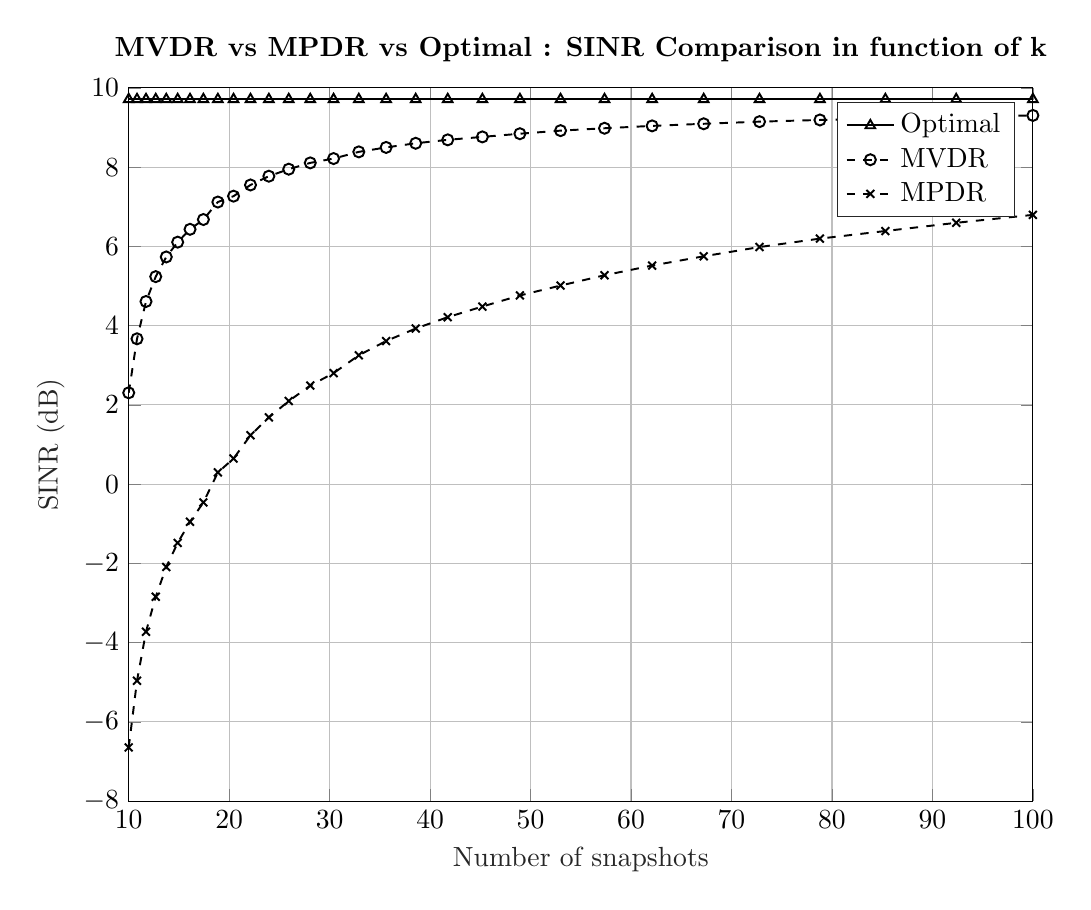
\begin{tikzpicture}

\begin{axis}[%
width=4.521in,
height=3.566in,
at={(0.758in,0.481in)},
scale only axis,
xmin=10,
xmax=100,
xlabel style={font=\color{white!15!black}},
xlabel={Number of snapshots},
ymin=-8,
ymax=10,
ylabel style={font=\color{white!15!black}},
ylabel={SINR (dB)},
axis background/.style={fill=white},
title style={font=\bfseries},
title={MVDR vs MPDR vs Optimal : SINR Comparison in function of k},
xmajorgrids,
ymajorgrids,
legend style={legend cell align=left, align=left, draw=white!15!black}
]
\addplot [color=black, line width=0.7pt, mark=triangle, mark options={solid, black}]
  table[row sep=crcr]{%
10	9.71005093279696\\
10.8263673387405	9.71005093279696\\
11.7210229753348	9.71005093279696\\
12.6896100316792	9.71005093279696\\
13.7382379588326	9.71005093279696\\
14.8735210729351	9.71005093279696\\
16.1026202756094	9.71005093279696\\
17.4332882219999	9.71005093279696\\
18.873918221351	9.71005093279696\\
20.4335971785694	9.71005093279696\\
22.1221629107045	9.71005093279696\\
23.9502661998749	9.71005093279696\\
25.9294379740467	9.71005093279696\\
28.0721620394118	9.71005093279696\\
30.391953823132	9.71005093279696\\
32.9034456231267	9.71005093279696\\
35.6224789026244	9.71005093279696\\
38.5662042116347	9.71005093279696\\
41.753189365604	9.71005093279696\\
45.2035365636024	9.71005093279696\\
48.9390091847749	9.71005093279696\\
52.9831690628371	9.71005093279696\\
57.3615251044868	9.71005093279696\\
62.1016941891562	9.71005093279696\\
67.2335753649934	9.71005093279696\\
72.7895384398315	9.71005093279696\\
78.8046281566991	9.71005093279696\\
85.3167852417281	9.71005093279696\\
92.3670857187387	9.71005093279696\\
100	9.71005093279696\\
};
\addlegendentry{Optimal}

\addplot [color=black, dashed, line width=0.7pt, mark=o, mark options={solid, black}]
  table[row sep=crcr]{%
10	2.30409725274647\\
10.8263673387405	3.66679128793078\\
11.7210229753348	4.60877459297854\\
12.6896100316792	5.23593547179515\\
13.7382379588326	5.73242597919632\\
14.8735210729351	6.10620127753702\\
16.1026202756094	6.4302740354056\\
17.4332882219999	6.67703250246094\\
18.873918221351	7.11857163454086\\
20.4335971785694	7.26674365957555\\
22.1221629107045	7.54948666188162\\
23.9502661998749	7.77082602948311\\
25.9294379740467	7.94807320050083\\
28.0721620394118	8.10664655811849\\
30.391953823132	8.21585888768401\\
32.9034456231267	8.384616428637\\
35.6224789026244	8.49676388370514\\
38.5662042116347	8.60156565874366\\
41.753189365604	8.6882916405326\\
45.2035365636024	8.76239500456989\\
48.9390091847749	8.84280656563659\\
52.9831690628371	8.92073099464416\\
57.3615251044868	8.98075835956239\\
62.1016941891562	9.04057306994228\\
67.2335753649934	9.09351345950654\\
72.7895384398315	9.14733724037471\\
78.8046281566991	9.18992308322662\\
85.3167852417281	9.22987092742139\\
92.3670857187387	9.26883916053122\\
100	9.30438494032605\\
};
\addlegendentry{MVDR}

\addplot [color=black, dashed, line width=0.7pt, mark=x, mark options={solid, black}]
  table[row sep=crcr]{%
10	-6.64585157676187\\
10.8263673387405	-4.96371583689953\\
11.7210229753348	-3.72631764831392\\
12.6896100316792	-2.8425644948737\\
13.7382379588326	-2.09094181839096\\
14.8735210729351	-1.4848790205482\\
16.1026202756094	-0.951878507044299\\
17.4332882219999	-0.463856092847431\\
18.873918221351	0.293711744498077\\
20.4335971785694	0.644754990622022\\
22.1221629107045	1.23066303468456\\
23.9502661998749	1.68170097249093\\
25.9294379740467	2.09522437671756\\
28.0721620394118	2.48606287145075\\
30.391953823132	2.80059019248449\\
32.9034456231267	3.25045162408333\\
35.6224789026244	3.61103133275049\\
38.5662042116347	3.92604737151289\\
41.753189365604	4.21261518771004\\
45.2035365636024	4.48088290006488\\
48.9390091847749	4.76101248930831\\
52.9831690628371	5.01047350082031\\
57.3615251044868	5.27028054795889\\
62.1016941891562	5.51591886151356\\
67.2335753649934	5.7489268680004\\
72.7895384398315	5.98284339428204\\
78.8046281566991	6.19547417406193\\
85.3167852417281	6.3874314037549\\
92.3670857187387	6.5943802756289\\
100	6.79431869223697\\
};
\addlegendentry{MPDR}

\end{axis}
\end{tikzpicture}%
        \caption{SINR in function of K}
        \label{fig:robust_k_sinr}
    \end{subfigure}\hspace{0.09\linewidth}
    \begin{subfigure}[b]{.4\linewidth}
        % This file was created by matlab2tikz.
%
%The latest updates can be retrieved from
%  http://www.mathworks.com/matlabcentral/fileexchange/22022-matlab2tikz-matlab2tikz
%where you can also make suggestions and rate matlab2tikz.
%
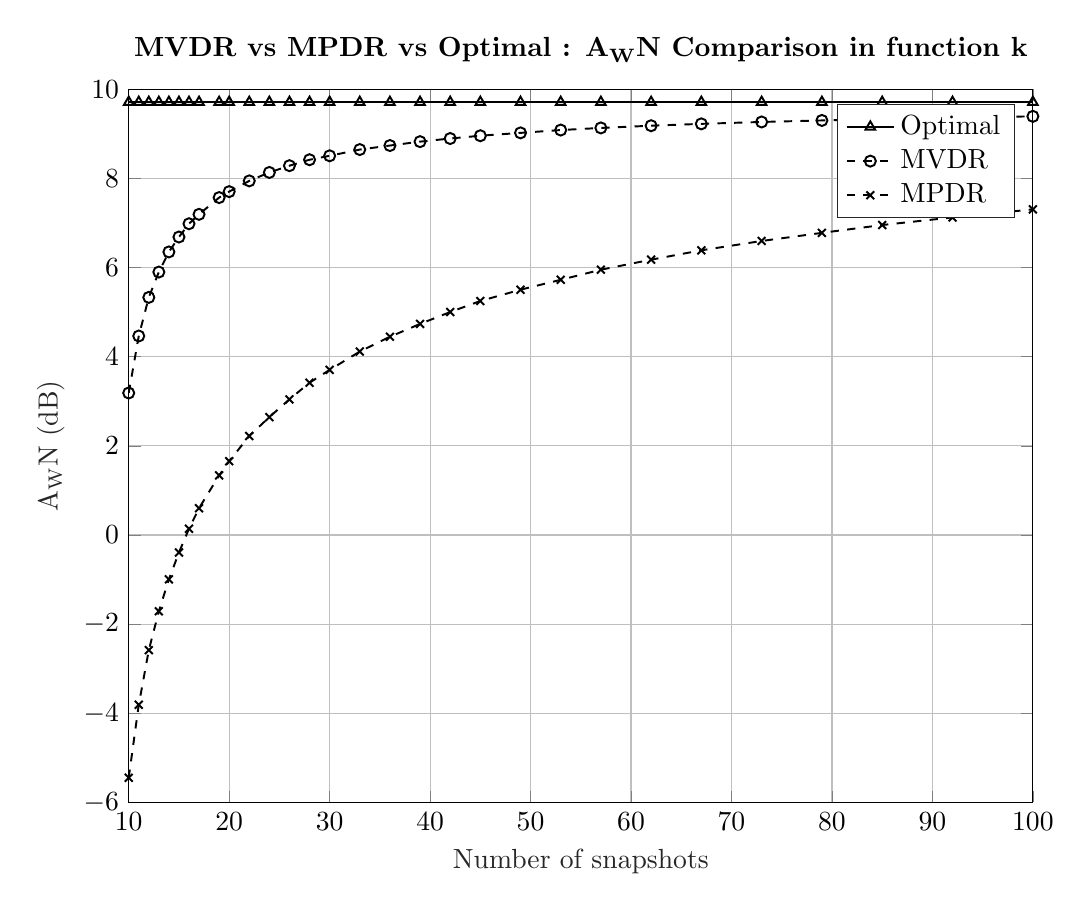
\begin{tikzpicture}

\begin{axis}[%
width=4.521in,
height=3.566in,
at={(0.758in,0.481in)},
scale only axis,
xmin=10,
xmax=100,
xlabel style={font=\color{white!15!black}},
xlabel={Number of snapshots},
ymin=-6,
ymax=10,
ylabel style={font=\color{white!15!black}},
ylabel={$\text{A}_\text{W}\text{N (dB)}$},
axis background/.style={fill=white},
title style={font=\bfseries},
title={$\text{MVDR vs MPDR vs Optimal : A}_\text{W}\text{N Comparison in function k}$},
xmajorgrids,
ymajorgrids,
legend style={legend cell align=left, align=left, draw=white!15!black}
]
\addplot [color=black, line width=0.7pt, mark=triangle, mark options={solid, black}]
  table[row sep=crcr]{%
10	9.71035096166968\\
11	9.71035096166968\\
12	9.71035096166968\\
13	9.71035096166968\\
14	9.71035096166968\\
15	9.71035096166968\\
16	9.71035096166968\\
17	9.71035096166968\\
19	9.71035096166968\\
20	9.71035096166968\\
22	9.71035096166968\\
24	9.71035096166968\\
26	9.71035096166968\\
28	9.71035096166968\\
30	9.71035096166968\\
33	9.71035096166968\\
36	9.71035096166968\\
39	9.71035096166968\\
42	9.71035096166968\\
45	9.71035096166968\\
49	9.71035096166968\\
53	9.71035096166968\\
57	9.71035096166968\\
62	9.71035096166968\\
67	9.71035096166968\\
73	9.71035096166968\\
79	9.71035096166968\\
85	9.71035096166968\\
92	9.71035096166968\\
100	9.71035096166968\\
};
\addlegendentry{Optimal}

\addplot [color=black, dashed, line width=0.7pt, mark=o, mark options={solid, black}]
  table[row sep=crcr]{%
10	3.1858273433172\\
11	4.46430883254148\\
12	5.33069434240174\\
13	5.89917927714449\\
14	6.35056601730387\\
15	6.68508365434538\\
16	6.98246746173726\\
17	7.19371909105452\\
19	7.56989854744007\\
20	7.70353047405681\\
22	7.94437324811085\\
24	8.1336767126934\\
26	8.28546291721345\\
28	8.41887417043098\\
30	8.50694762334552\\
33	8.64703760525257\\
36	8.73722616131266\\
39	8.82469204056024\\
42	8.89480221796905\\
45	8.95704129914239\\
49	9.02147385710691\\
53	9.08470026274564\\
57	9.13230257627051\\
62	9.18178793872922\\
67	9.22380215822138\\
73	9.26626234117354\\
79	9.30018479224346\\
85	9.33218758455842\\
92	9.36301745880865\\
100	9.39214072101658\\
};
\addlegendentry{MVDR}

\addplot [color=black, dashed, line width=0.7pt, mark=x, mark options={solid, black}]
  table[row sep=crcr]{%
10	-5.44741313972959\\
11	-3.8092155456058\\
12	-2.58310669360123\\
13	-1.71048222963139\\
14	-0.993965520436374\\
15	-0.392786759782729\\
16	0.139498094738418\\
17	0.601260573494368\\
19	1.33653077444616\\
20	1.65552169298704\\
22	2.22176624523533\\
24	2.64572673449262\\
26	3.04232664109941\\
28	3.41673529268007\\
30	3.70449479978281\\
33	4.11494729937684\\
36	4.44759381046901\\
39	4.73552675684083\\
42	5.00181694919012\\
45	5.24970617488015\\
49	5.5031717217801\\
53	5.72536132117846\\
57	5.95140930684828\\
62	6.17666267392546\\
67	6.3870488432302\\
73	6.59603766233756\\
79	6.77828669297885\\
85	6.95411162846517\\
92	7.1244031202874\\
100	7.3054238990382\\
};
\addlegendentry{MPDR}

\end{axis}
\end{tikzpicture}%
        \caption{$A_{WN}$ in function of K}
        \label{fig:robust_k_awn}
    \end{subfigure}
    \caption{Convergence in function of K of MVDR and MPDR.}
    \label{fig:mpdr_robust}
\end{figure}

It appears from both figures \ref{fig:robust_k_sinr} and \ref{fig:mpdr_robus_awn} that MPDR requires way more snapshots than MVDR to converge. 

\end{document}